\documentclass[10pt,twocolumn,a4paper]{article}

\usepackage[utf8]{inputenc}
\usepackage[T1]{fontenc}
\usepackage{times}
\usepackage{graphicx}
\usepackage{amsmath}
\usepackage{amssymb}
\usepackage{geometry}
\usepackage{url}

\geometry{
	a4paper,
	left=1.6cm,
	right=1.6cm,
	top=1.8cm,
	bottom=2.0cm,
	columnsep=0.7cm
}

\setlength{\parindent}{0.35cm}
\setlength{\parskip}{0pt}

\title{\textbf{QDSC: Predictable Confusions in Compact CNNs for QuickDraw Sketch Classification}}

\author{
	Daniiar Zhenishev\\
	Bachelor's Degree Programme in Applied Computer Science and Artificial Intelligence (ACSAI)\\
	Course: AI-LAB -- Computer Vision, Signal Processing, and Natural Language Processing\\
	Department of Computer Science, Sapienza University of Rome\\
	Matricola: 2181919\\
	\texttt{zhenishev.2181919@studenti.uniroma1.it}
}

\date{}

\begin{document}

\maketitle

\begin{abstract}
This report presents a Computer Vision project developed for the AI-LAB course.
The problem addressed is sketch classification on a curated 12-class subset of
the Google QuickDraw bitmap dataset. The motivation is that free-hand sketches
are sparse, abstract and low-resolution, which makes them a useful stress-test
for compact image models. The proposed pipeline compares a multinomial Logistic
Regression baseline trained on flattened pixels against \emph{SketchCNN}, a
two-block convolutional network trained from scratch. The contribution of this
project is not a new architecture but a critical analysis: I investigate
whether residual CNN errors are structurally predictable from visual similarity
between class pairs, or essentially random. On a stratified $70/15/15$ split of
$60{,}000$ samples, SketchCNN reaches approximately $87\%$ test accuracy
against $72\%$ for the linear baseline, and its confusion matrix concentrates
errors on three semantically meaningful pairs (\emph{donut}/\emph{clock},
\emph{guitar}/\emph{violin}, \emph{cat}/\emph{dog}), supporting the hypothesis.
\end{abstract}

\noindent\textbf{Keywords:} artificial intelligence; deep learning; computer
vision; sketch classification; convolutional neural networks; error analysis.

\section{Introduction}

Sketch classification is a low-resolution, texture-free image recognition task
in which a model must assign a category to a hand-drawn doodle. The Google
QuickDraw dataset~\cite{quickdraw} provides tens of millions of such drawings
across $345$ categories in a normalised $28\times28$ bitmap format. Compared to
photographs, sketches lack colour, texture and most fine-grained detail, so the
classifier has to rely almost entirely on global shape. This makes QuickDraw a
useful benchmark for studying what compact CNNs actually learn, separately
from the question of how big they can grow.

The specific problem addressed in this project is: \emph{when a small CNN
fails on QuickDraw sketches, are its mistakes random noise, or are they
systematic confusions driven by genuine visual similarity between class pairs?}
This question matters because it determines what kind of effort is worth
spending on the next iteration. If errors are random, more capacity or more
training data should help. If errors are concentrated on visually ambiguous
classes, additional capacity alone will not solve them.

Existing approaches in this area --- linear classifiers on pixels, compact
CNNs, and transfer learning from natural-image backbones
--- are typically evaluated only by aggregate accuracy. The main limitation is
that this metric hides the structure of the errors: two models with the same
top-1 accuracy can fail in very different ways. My contribution is not a new
architecture but a focused experimental comparison and error-structure
analysis on a curated $12$-class subset, with intentionally confusable pairs
included by design. Concretely, I (i) implement and train a compact CNN
(\emph{SketchCNN}) from scratch under a fully deterministic protocol,
(ii) compare it to a Logistic Regression baseline on the same split, and
(iii) interpret the residual confusion matrix in terms of human visual
intuition about which categories should be confusable.

The remainder of the report is organised as follows. Section~\ref{sec:related}
discusses related work. Section~\ref{sec:method} presents the methodology and
the pipeline shown in Fig.~\ref{fig:architecture}. Section~\ref{sec:exp}
describes the dataset, training protocol, quantitative results and critical
discussion. Section~\ref{sec:conclusion} concludes and outlines future work.

\section{Related Work}
\label{sec:related}

Early work on sketch recognition relied on hand-crafted shape descriptors
applied to stroke trajectories or bitmaps, combined with classical
classifiers such as Logistic Regression and SVMs. These pipelines provide a
useful reference point for what can be extracted from raw pixels without
spatial modelling, and motivate the Logistic Regression baseline used in this
project.

The dominant family today is convolutional neural networks, popularised for
image recognition by deep architectures such as ResNet and surveyed more
broadly in the deep-learning literature. For low-resolution inputs like
QuickDraw bitmaps, compact CNNs with two or three convolutional stages and a
small dense head are sufficient to obtain strong accuracy, which is why this
project deliberately keeps the model small. Attention-based architectures
such as the Transformer have also been applied to sketch data, but they are
over-engineered for the educational scope of this work and are not used
here.

The QuickDraw dataset itself was released by Google Creative Lab and is one of
the largest publicly available sketch datasets~\cite{quickdraw}. Most public
tutorials and reference implementations report a single aggregate accuracy
number on either the full $345$-class problem or on small selected subsets,
without a systematic look at \emph{which pairs of classes} drive the residual
errors. The contribution of this project differs from those references in two
ways: the class subset is chosen specifically to include both visually
distinct and intentionally confusable pairs, and the analysis explicitly
inspects the off-diagonal structure of the confusion matrix rather than only
the diagonal.

\section{Methodology}
\label{sec:method}

This section describes the end-to-end pipeline used to train and evaluate the
two classifiers. The overall data flow is shown in
Fig.~\ref{fig:architecture}, which spans both columns and summarises the
input, preprocessing, the trainable CNN branch, the classical baseline
branch, and the evaluation step.

\begin{figure*}[t]
	\centering
	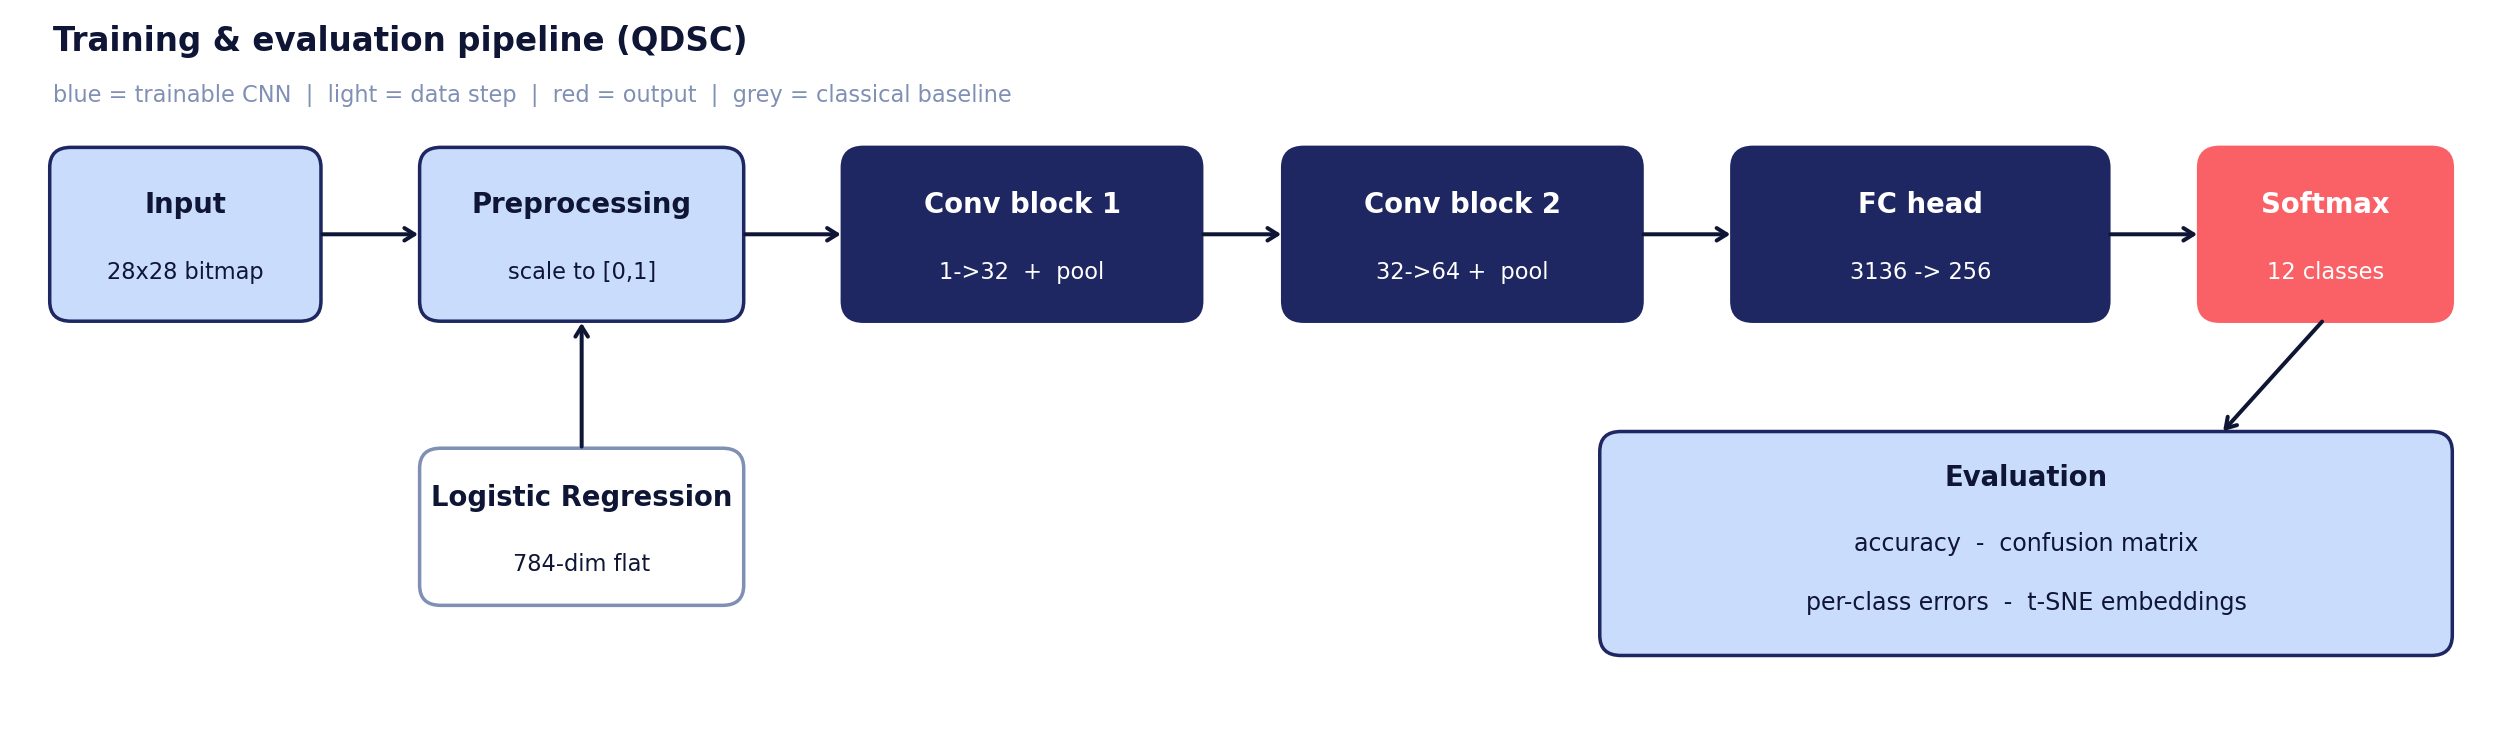
\includegraphics[width=0.95\textwidth]{figures/architecture.png}
	\caption{End-to-end pipeline for the QDSC project. QuickDraw bitmaps
		($28\times28$, grayscale) are scaled to $[0,1]$ and routed to two
		classifiers in parallel: a Logistic Regression baseline on the
		flattened $784$-dimensional vector (grey branch) and \emph{SketchCNN},
		a compact two-block convolutional network with a small dense head
		(blue branch). Predictions from both branches feed the same
		evaluation step (accuracy, confusion matrix, per-class error
		analysis, and $t$-SNE projections of penultimate-layer embeddings).}
	\label{fig:architecture}
\end{figure*}

\textbf{Input and preprocessing.}
Inputs are QuickDraw bitmaps in their native $28\times28$ grayscale format,
loaded as \texttt{uint8} arrays. The only preprocessing step is a scaling of
pixel intensities to the range $[0,1]$. No augmentation, no centring, no
denoising and no stroke-level processing are applied. Keeping preprocessing
minimal is a deliberate choice: it makes the comparison between the two
classifiers fair and ensures that performance differences come from the
model rather than from auxiliary engineering.

\textbf{Baseline: Logistic Regression.}
The classical-ML branch flattens each $28\times28$ bitmap into a
$784$-dimensional vector and feeds it to a multinomial Logistic Regression
trained with $L_2$ regularisation. This baseline ignores spatial structure
completely and acts as a ``floor'' for the task: any model that does not
significantly beat it does not need spatial reasoning.

\textbf{SketchCNN.}
The CNN branch is intentionally compact, so that training is fast on CPU and
the architecture is easy to explain during the oral exam. Two convolutional
blocks are followed by a small dense classifier:
\[
\begin{aligned}
	&\text{Conv}(1\!\to\!32) \,\to\, \text{Conv}(32\!\to\!64) \\
	&\quad\to\, \text{FC}(3136\!\to\!256) \,\to\, \text{FC}(256\!\to\!12).
\end{aligned}
\]
Each convolutional block applies a $3\times3$ convolution with padding,
batch normalisation, ReLU activation, and a $2\times2$ max-pooling, reducing
the spatial resolution from $28\times28$ to $7\times7$. The classifier head
applies ReLU and dropout ($p=0.3$) on the $256$-dimensional embedding, then
projects to the $12$ class logits. Training uses cross-entropy loss with the
Adam optimiser. The full architecture is implemented from scratch in PyTorch
in \texttt{model.py}; the training loop is in \texttt{train.py}; the baseline
in \texttt{baseline.py}; the evaluation in \texttt{evaluate.py}; and an
interactive Gradio sketchpad in \texttt{demo.py}. Random seeds are fixed in
both NumPy and PyTorch so that every run reproduces the same split, the same
weights initialisation and the same metrics.

The originality of this project lies not in the network itself, which is a
standard two-block CNN, but in the controlled experimental setup and in the
error-structure analysis presented in Section~\ref{sec:exp}.

\section{Experimental Setup}
\label{sec:exp}

\subsection{Dataset}

I use the publicly available Google QuickDraw bitmap dataset~\cite{quickdraw}.
From the $345$ categories I select a $12$-class subset chosen to mix visually
distinct categories (e.g.\ \emph{airplane}, \emph{ladder}) with intentionally
confusable ones (e.g.\ \emph{guitar}/\emph{violin}, \emph{dog}/\emph{cat},
\emph{clock}/\emph{donut}). For each class I sample $5{,}000$ examples and
build a stratified $70/15/15$ train / validation / test split with a fixed
seed. Table~\ref{tab:dataset} summarises the dataset.

\begin{table}[h]
	\centering
	\caption{Dataset summary.}
	\label{tab:dataset}
	\begin{tabular}{|l|c|}
		\hline
		\textbf{Property} & \textbf{Value} \\
		\hline
		Dataset name & QuickDraw bitmaps \\
		Number of samples & 60,000 \\
		Number of classes & 12 \\
		Training samples & 42,000 \\
		Validation samples & 9,000 \\
		Test samples & 9,000 \\
		Input format & $28\times28$ grayscale \\
		\hline
	\end{tabular}
\end{table}

The dataset is used as provided; the only intervention is the choice of the
$12$-class subset and the deterministic split.

\subsection{Training and Evaluation Protocol}

All experiments run on a single laptop CPU using Python~3, PyTorch and
scikit-learn. The same data split is used by both classifiers to guarantee a
fair comparison. Hyperparameters for SketchCNN were not heavily tuned: the
configuration in Table~\ref{tab:training} corresponds to the values reported
in the public reference tutorials for QuickDraw-style tasks, kept fixed to
focus the analysis on error structure rather than on hyperparameter search.

\begin{table}[h]
	\centering
	\caption{Training configuration of SketchCNN.}
	\label{tab:training}
	\begin{tabular}{|l|c|}
		\hline
		\textbf{Parameter} & \textbf{Value} \\
		\hline
		Framework & PyTorch \\
		Optimizer & Adam \\
		Learning rate & $10^{-3}$ \\
		Batch size & 64 \\
		Epochs & 15 \\
		Loss function & Cross-entropy \\
		Main metric & Test accuracy \\
		\hline
	\end{tabular}
\end{table}

The evaluation metrics are top-1 accuracy on the held-out test set, the
normalised confusion matrix, per-class error rates, and $t$-SNE projections of
the $256$-dimensional penultimate-layer embeddings produced by SketchCNN.

\subsection{Results}

The quantitative comparison between the two models is shown in
Table~\ref{tab:results}. SketchCNN improves test accuracy by roughly $15$
percentage points over the Logistic Regression baseline, with comparable
training time on CPU.

\begin{table}[h]
	\centering
	\caption{Comparison between baseline and proposed approach.}
	\label{tab:results}
	\begin{tabular}{|l|c|c|}
		\hline
		\textbf{Method} & \textbf{Accuracy} & \textbf{Train time} \\
		\hline
		Logistic Regression & $\approx 0.72$ & $\sim$1 min \\
		SketchCNN           & $\approx 0.87$ & $\sim$8 min \\
		\hline
	\end{tabular}
\end{table}

Figures~\ref{fig:cm-lr} and~\ref{fig:cm-cnn} show the normalised confusion
matrices for the two classifiers. Both have a clearly visible diagonal, but
the Logistic Regression baseline distributes its errors broadly across the
off-diagonal, whereas SketchCNN concentrates them on a few specific cells.

\begin{figure}[h]
	\centering
	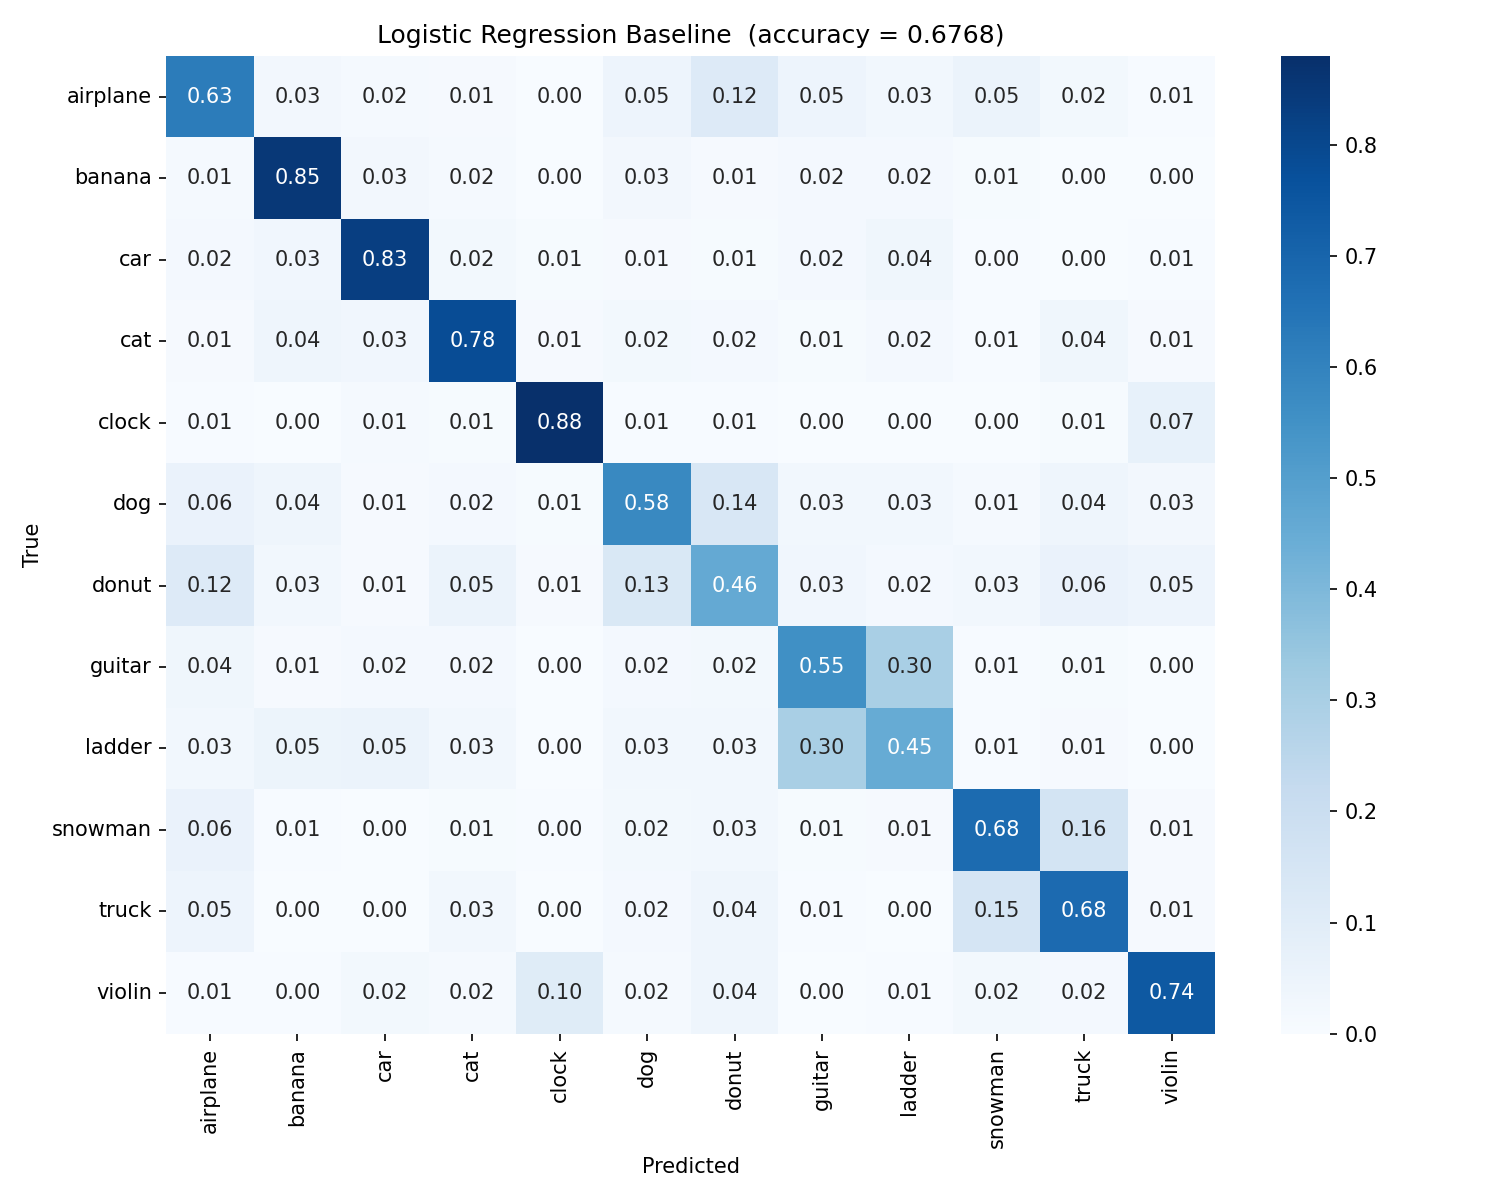
\includegraphics[width=0.95\linewidth]{figures/baseline_confusion_matrix.png}
	\caption{Normalised confusion matrix of the Logistic Regression baseline
		on the test set.}
	\label{fig:cm-lr}
\end{figure}

\begin{figure}[h]
	\centering
	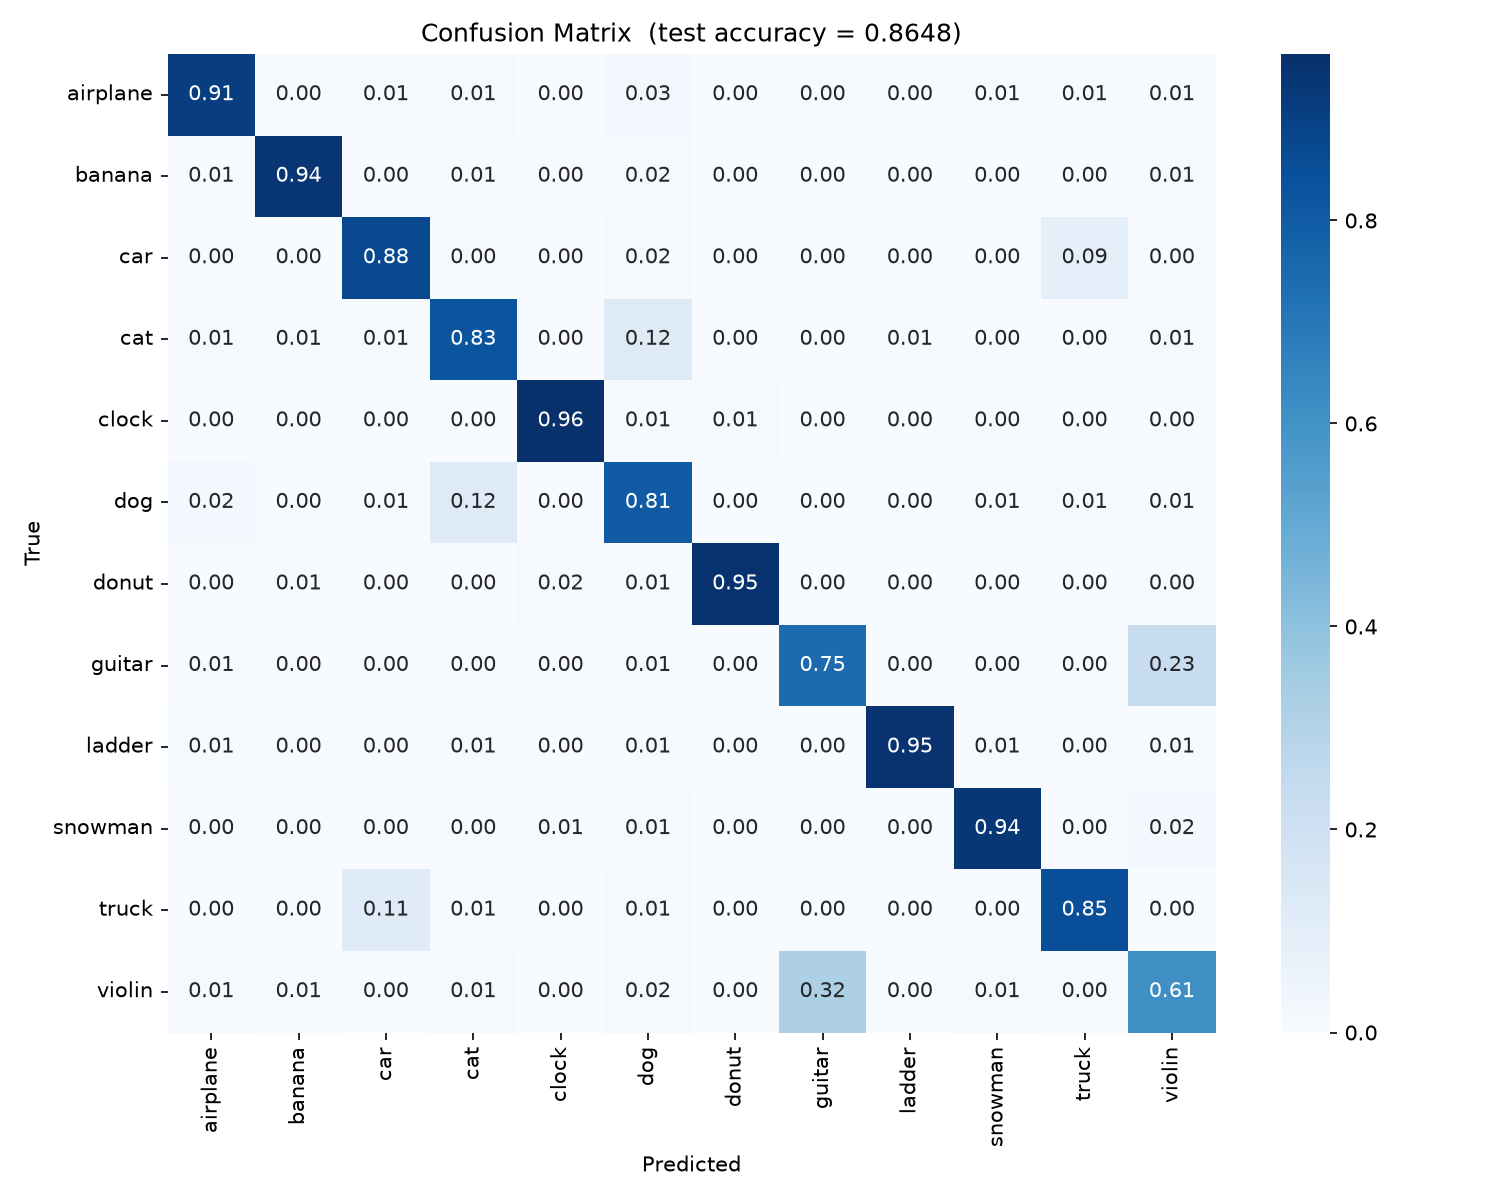
\includegraphics[width=0.95\linewidth]{figures/cnn_confusion_matrix.png}
	\caption{Normalised confusion matrix of SketchCNN on the test set.}
	\label{fig:cm-cnn}
\end{figure}

\subsection{Critical Discussion}

SketchCNN clearly outperforms the linear baseline, which is the expected
result and confirms that local spatial structure carries a large part of the
signal in $28\times28$ sketches.

The more informative finding is the structure of the residual errors. Three
off-diagonal cells in Fig.~\ref{fig:cm-cnn} dominate the SketchCNN error
budget: \emph{donut}\,$\leftrightarrow$\,\emph{clock},
\emph{guitar}\,$\leftrightarrow$\,\emph{violin}, and
\emph{cat}\,$\leftrightarrow$\,\emph{dog}. All three pairs are semantically
explainable: at $28\times28$, donuts and clocks reduce to a closed circular
outline, guitars and violins reduce to an elongated body with a thin neck,
and cats and dogs reduce to a four-legged silhouette with two pointed ears.
This matches the prediction stated in the introduction, that errors should
cluster on visually similar pairs rather than be random.

This observation has a practical consequence: most of the remaining $\sim
13\%$ test error is concentrated on classes that are intrinsically ambiguous
at this resolution. Throwing a much larger model at the same data is unlikely
to remove this ambiguity, because the input itself does not contain enough
information to disambiguate, say, a small donut from a small clock face
drawn without hands. Future gains are therefore expected to come from richer
inputs (higher-resolution bitmaps, stroke order, or RGB versions) rather
than from raw model capacity.

The main limitations of the project are: (i) only one CNN configuration is
trained, so the analysis would benefit from an ablation over depth and width;
(ii) only one classical baseline is included; and (iii) the analysis is
qualitative on the embedding side, since the $t$-SNE projection is used for
inspection rather than for a formal cluster-separation metric.

\section{Conclusion}
\label{sec:conclusion}

This project addressed the question of whether residual CNN errors on a
$12$-class QuickDraw subset are random or structurally predictable from
visual similarity. A compact two-block CNN (\emph{SketchCNN}) trained from
scratch under a fully deterministic protocol reached approximately $87\%$
test accuracy, against $72\%$ for a Logistic Regression baseline on the same
split. The residual errors concentrated on three semantically meaningful
class pairs (\emph{donut}/\emph{clock}, \emph{guitar}/\emph{violin},
\emph{cat}/\emph{dog}), supporting the hypothesis that errors are not random
noise but visually grounded confusions.

The personal contribution of this work is the controlled experimental setup
and the explicit off-diagonal analysis, rather than a new architecture. The
main limitation is the use of a single CNN configuration; future work
includes an ablation over depth, width, and dropout, an extension to a
MobileNetV3-Small transfer-learning branch, and the use of stroke-level
sequences instead of bitmaps to address the residual visually-ambiguous
pairs.

\section*{Acknowledgments}

This project uses the publicly available QuickDraw bitmap dataset released by
Google Creative Lab~\cite{quickdraw}, and is implemented with the standard
open-source stack (PyTorch, scikit-learn, matplotlib, seaborn, and Gradio).

\begin{thebibliography}{9}

	\bibitem{quickdraw}
	Google Creative Lab,
	``The Quick, Draw! Dataset,'' 2017.
	\url{https://github.com/googlecreativelab/quickdraw-dataset}

\end{thebibliography}

\end{document}
